\section{Additional Related Work}

%Due to page limitations, we have included the complete version of the related work in Appendix \ref{apd:Additional Related Work}. Graphs effectively represent complex relationships using nodes and edges, with Graph Neural Networks (GNNs) \citep{fey2023relational,cao2023relational,gao2020ci,chen2022gndan,wu2022graph,yang2021consisrec, Thomas2017GCN,hamilton2017graphsage,velivckovic2017gat,schlichtkrull2017modeling} emerging as the preferred technology for applications in recommendation systems \citep{Erxue2022recommender} and social networks \citep{wu2020social}. GNNs, particularly with advancements like the GFM \citep{chen2024llaga,liu2023one}, address challenges such as the cold start problem by leveraging zero-shot or few-shot learning capabilities. Concurrently, WMs \citep{ha2018recurrent} have evolved to predict future states from unstructured data, with implementations like Genie \citep{bruce2024genie} using serialized internet videos for planning. However, these models struggle to effectively incorporate structured data into their predictions.  Our integration of graph technologies into the WM allows it to generalize across diverse tasks such as prediction, generation, and planning.




\xhdr{Graph for Modelling Relations} Graphs are highly effective in modeling complex relationships \citep{fey2023relational,cao2023relational,gao2020ci,chen2022gndan,wu2022graph,yang2021consisrec}, extracting nodes and edges to model relational data with embeddings. Graph Neural Networks (GNNs) \citep{Thomas2017GCN,hamilton2017graphsage,velivckovic2017gat,schlichtkrull2017modeling} have emerged as a dominant approach, particularly in recommendation systems \citep{Erxue2022recommender} and social networks \citep{wu2020social}. To further address the vast array of tasks and data, scholars have proposed the GFM \citep{chen2024llaga,liu2023one} to explore GNNs' zero-shot or few-shot capabilities \citep{fey2023relational,cao2023relational,gao2020ci,chen2022gndan} to tackle challenges such as the cold start problem in recommendations. 

%\vspace{-3mm}
%\vspace{-1mm}
\begin{figure}[t]
\centering
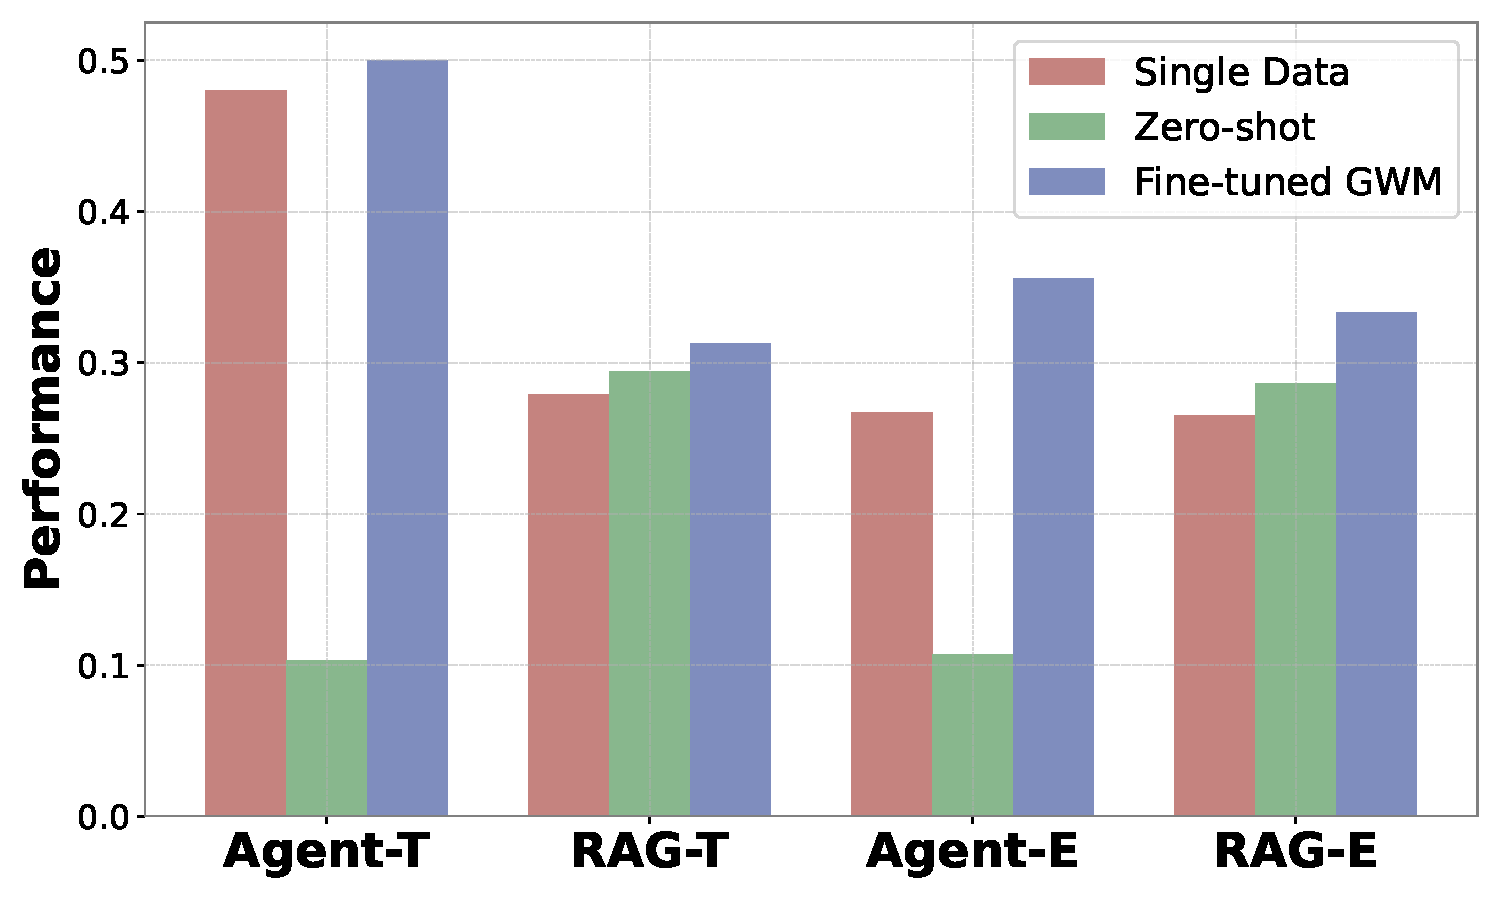
\includegraphics[width=\linewidth]{figs/zero_few_shot.pdf} 
\caption{\textbf{GWM boosts zero-shot/few-shot performance on multi-agent collaboration (Agent) and retrieval-augmented generation (RAG) tasks}. Note that ``-T'' and ``-E'' respectively represent the experimental results of GWM-T and GWM-E. It can be observed that  GWM can quickly adapt to new tasks with a small amount of domain-specific training data. Moreover, GWM's strong generalization ability can boost the performance of Agent and RAG.} %It can be observed that  GWM can quickly adapt to new tasks with a small amount of domain-specific training data. Moreover, GWM's strong generalization ability can boost the performance of Agent and RAG.
\label{fig:zero_few_shot}
\end{figure}
% \vspace{-3mm}
% \vspace{-3mm}

\xhdr{World Model} The WM \citep{ha2018recurrent} is to construct the world observations as states and predict future states based on given actions. Existing WMs \citep{wu2024ivideogpt,bruce2024genie} primarily focus on how to utilize unstructured data to predict state transitions, thereby enhancing the effectiveness of sequence generation tasks. Genie \citep{bruce2024genie} trained a foundation world model using a massive amount of unlabelled, serialized internet videos, which has provided benefits for the planning outcomes of downstream tasks. Additionally, some WMs \citep{zhang2021world,zhu2022value} have attempted to integrate structured data with GWM. $L^3P$ \citep{zhang2021world} uses graphs to model each step of the agent's decision-making process and their connections, thus enhancing scalable planning in reinforcement learning. However, they are still largely confined to planning and optimization scenarios, which limits their potential for task generalization as WMs. Thus we  develop GWM that integrates the capabilities of graphs with WM to generalize across diverse tasks.










